\Askhsh{38862}{4}
\begin{ylh}{2}
    \item 6.2. Γραφική Παράσταση Συνάρτησης
    \item 6.3. Η Συνάρτηση $f(x)=ax+\beta$
\end{ylh}

Οι επιστήμονες παρακολουθούν το λιώσιμο ενός παγετώνα λόγω της κλιματικής αλλαγής. Η συνάρτηση που εκφράζει τον όγκο του παγετώνα $V(t)$ ως συνάρτηση του χρόνου $t$ δίνεται από τον τύπο $V(t) = 4500 - 15t$, όπου $t$ είναι τα έτη μετά το $2020$, π.χ. το $t = 5$ δηλώνει το 2025.
\begin{alist}
\item Να περιγράψετε τι εκφράζουν, στο πλαίσιο του προβλήματος, οι αριθμοί $4500$ και $15$ στον τύπο της συνάρτησης $V(t)$.
\monades{3}
\item Να υπολογίσετε ποιος περίπου θα είναι ο όγκος του παγετώνα το έτος $2040$.
\monades{5}
\item Να υπολογίσετε σε ποιο έτος ο όγκος του παγετώνα θα πέσει κάτω από $500\ m^{3}$, αν συνεχιστεί ο ίδιος ρυθμός λιωσίματος που παρατήρησαν οι επιστήμονες.
\monades{6}
\item
\begin{rlist}
\item Να μεταφέρετε στην κόλλα σας το παρακάτω σύστημα αξόνων και να σχεδιάσετε σε αυτό τη γραφική παράσταση της συνάρτησης $V(t)$ ως συνάρτηση του $t$.
\begin{center}
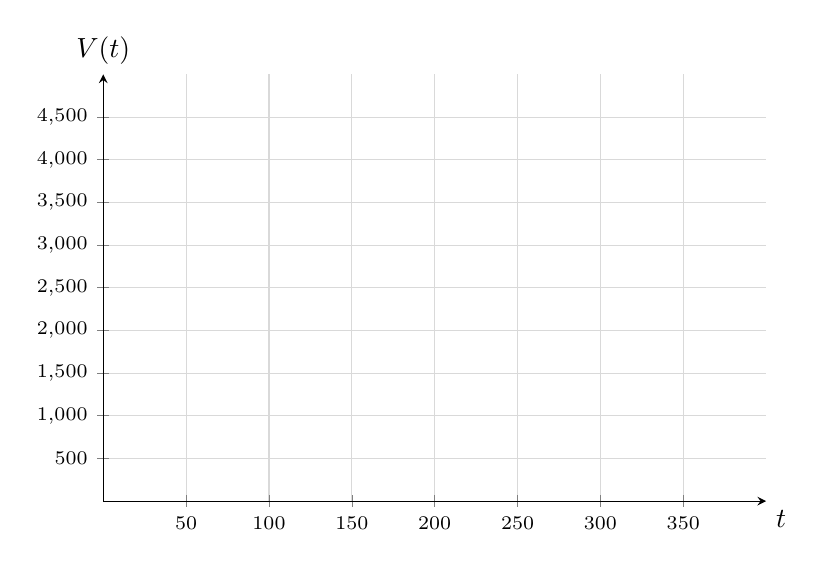
\begin{tikzpicture}
\begin{axis}[
    axis lines = left,
    xlabel = {$t$},
    ylabel = {$V(t)$},
    xmin = 0, xmax = 400,
    ymin = 0, ymax = 5000,
    xtick = {50,100,150,200,250,300,350},
    ytick = {500,1000,1500,2000,2500,3000,3500,4000,4500},
    grid = both,
    grid style = {gray!30},
    width = 10cm, height = 7cm,
    tick label style = {font=\scriptsize},
    every axis x label/.style = {at={(current axis.right of origin)}, anchor=north west},
    every axis y label/.style = {at={(current axis.above origin)}, anchor=south},
]
\end{axis}
\end{tikzpicture}\captionof{figure}{Άσκηση 38862}
\end{center}

\monades{4}
\item Να ελέγξετε αν το σημείο $(300, 0)$ είναι σημείο της γραφικής παράστασης της συνάρτησης.
\monades{3}
\item Αν ναι, να ερμηνεύσετε το σημείο αυτό στο πλαίσιο του προβλήματος που αφορά τον όγκο του παγετώνα και το λιώσιμο των πάγων.
\monades{4}
\end{rlist}
\end{alist}

